% ****** Start of file aipsamp.tex ******
%
%   This file is part of the AIP files in the AIP distribution for REVTeX 4.
%   Version 4.1 of REVTeX, October 2009
%
%   Copyright (c) 2009 American Institute of Physics.
%
%   See the AIP README file for restrictions and more information.
%
% TeX'ing this file requires that you have AMS-LaTeX 2.0 installed
% as well as the rest of the prerequisites for REVTeX 4.1
% 
% It also requires running BibTeX. The commands are as follows:
%
%  1)  latex  aipsamp
%  2)  bibtex aipsamp
%  3)  latex  aipsamp
%  4)  latex  aipsamp
%
% Use this file as a source of example code for your aip document.
% Use the file aiptemplate.tex as a template for your document.
\documentclass[%
 aip,
 % onecolumn,
% jmp,
% bmf,
% sd,
 % rsi,
 amsmath,amssymb,
%preprint,%
 reprint,%
%author-year,%
%author-numerical,%
% Conference Proceedings
floatfix,
% tikz,
]{revtex4-1}

\usepackage{graphicx}% Include figure files
\usepackage[utf8]{inputenc}
\usepackage[T1]{fontenc}
\usepackage{mathptmx}
\usepackage{tikz}
\usetikzlibrary{arrows,decorations.markings,decorations.pathmorphing, patterns,shapes}
\usepackage{dcolumn}% Align table columns on decimal point
\usepackage{bm}% bold math
\usepackage{float}
%\usepackage[mathlines]{lineno}% Enable numbering of text and display math
%\linenumbers\relax % Commence numbering lines

\begin{document}
\preprint{AIP/123-QED}

\title[]{The Lifetime of the Muon}
% Force line breaks with \\

\author{Jared Baur and Ben Sappey}
 % \altaffiliation[Also at ]{Physics Department, XYZ University.}%Lines break automatically or can be forced with \\
% \author{Ben Sappey}%
% \affiliation{ 
% Authors' institution and/or address%\\This line break forced with \textbackslash\textbackslash
% }%

\date{\today}% It is always \today, today,
             %  but any date may be explicitly specified


\begin{abstract}

	Insert abstract here.

\end{abstract}

\maketitle


\onecolumngrid

\section{\label{sec:level1}Objective}

To determine the lifetime of the muon.

\section{\label{sec:level2}Introduction}

The muon was first discovered in 1936 by Carl D. Anderson and Seth Neddermeyer. They were studying cosmic radiation when Anderson noticed that certain particles curved differently from the known particles passing through a magnetic field. The negatively charged particles curved less sharply than electrons and more sharply than protons, but all carried the same velocity through the magnetic field. Originally, the charge of this particle was assumed to be of the same negative magnitude as electrons, and thus the difference in curvature was explained by giving this particle a mass greater than an electron and less than a proton. This particle was originally called a “mesotron”, the “meso” prefix meaning “middle”, as in having a mass between that of an electron or proton. Later in 1947, a particle with similar mass but dissimilar force properties was discovered. These two particles were grouped together as “mesons” instead of mesotrons (still meaning they have an intermediate mass to electrons and protons). The particle discovered in 1947 by Yukawa is now known as the $\pi$-meson. The previous meson mentioned is called the $\mu$-meson, or the muon.

The decay of a muon is in accordance to the radioactive decay law, which states that the probability of decay for a small increment of time $\delta t$ is stated in Equation 1. The constant $\lambda$ is the decay rate, which results in a constant probability of decay. This means that the probability of decay does not change over the lifetime of the muon, as may contradict common sense of this probability increasing as the lifetime increases.

\begin{equation}
	P(\delta t) = \lambda \delta t
\end{equation}

When a muon decays, it splits into separate particles; the muon $\mu^-$ and the antimuon $\mu^+$ decay into the particles given by Equation 2. The variables $\nu_e$ and $\nu_\mu$ are neutrinos with small mass that only interact with the weak and gravitational forces; their respective antiparticles are $\bar{\nu}_e$ and $\bar{\nu}_\mu$.

\begin{equation}
	\begin{aligned}
		\mu^- \rightarrow e^- + \nu_e + \bar{\nu}_\mu \indent \text{(100\%)} \\
		\mu^+ \rightarrow e^+ + \bar{\nu}_e + \nu_\mu \indent \text{(100\%)}
	\end{aligned}
\end{equation}

\section{\label{sec:level3}Apparatus and Methods}

\begin{figure}[H]
	\centering
	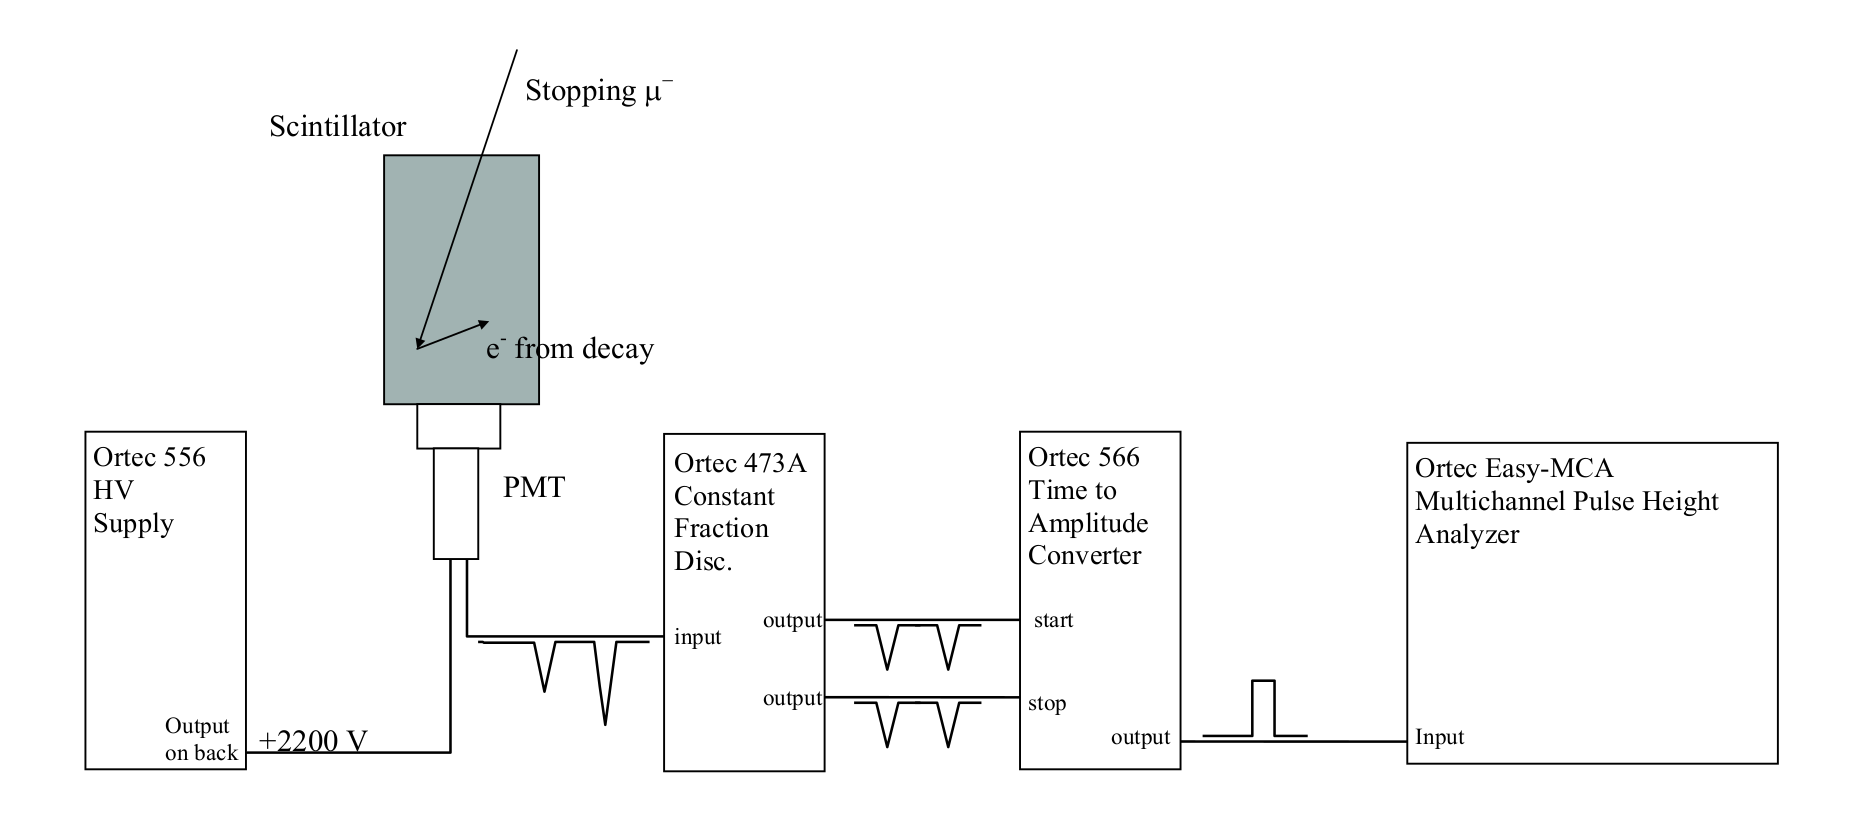
\includegraphics[scale=0.25]{schematic.png}
	\caption{}
\end{figure}

In order to perform this experiment, a continuous source of muons is required. This supply of muons is available from the constant raining of cosmic rays on Earth's atmosphere. These high enery cosmic ray protons enter the upper atmosphere and collide with nuclei A, resulting in pion particles (Equation 3).

\begin{equation}
	p + A \rightarrow \pi^{\pm}, \pi^0
\end{equation}

These pions decay and produce the particles listed in Equation 4.

\begin{equation}
	\begin{aligned}
		\pi^+ & \rightarrow \mu^+ + \nu_{\mu} \\
		\pi^- & \rightarrow \mu^- + \bar{\nu}_{\mu} \\
		\pi^0 & \rightarrow 2\lambda
	\end{aligned}
\end{equation}



\subsection{Calibration}

Calibration of the apparatus was completed in two steps. First, the discriminator was calibrated by using a pulse generator to send of pulses of a fixed amplitude to the discriminator. The signal from the pulse generator was connected to the discriminator input using a T-connector, which was then routed to the oscilloscope. The discriminator was adjusted so that the pulses were output to the screen of the oscilloscope with minimal noise. This process was repeated for various pulse amplitudes in order to find a proper discriminator value for differing conditions.

The next step of calibration was for the MCA time scale. The pulse generator was set to output two pulses at a time $\Delta t$ apart. The “measure” menu on the oscilloscope allows for easy measurement of this time separation. These dual pulse signals were then sent to the discriminator, which would thus filter the signals based on the time separation, not the amplitude of the pulse. The discriminator was set so that the oscilloscope consistently gave an output.

\section{\label{sec:level4}Data Analysis}


\section{\label{sec:level5}Conclusion}


\nocite{*}
\bibliography{main}% Produces the bibliography via BibTeX.
\end{document}
